%!TeX spellcheck = pt_BR
\documentclass[brazil]{beamer}
%\usepackage[timeinterval=1,font=Helv]{tdclock}
\usetheme{Frankfurt}
\useoutertheme[subsection=false,footline=authortitle]{miniframes}
%\useoutertheme{shadow}


%\usepackage{beamerthemesplit}
%\usepackage{ragged2e}
%\usepackage{etoolbox}
\usepackage{hyphenat}
\usepackage{babel}
%\hyphenation{mate-mática recu-perar}
\usepackage[T1]{fontenc}
\usepackage{lmodern}
\usepackage[utf8x]{inputenc}
\usepackage[figurename=Imagem]{caption}
\usepackage[alf,abnt-etal-cite=2]{abntex2cite}
%\usepackage{remreset}
%\makeatletter
%\@removefromreset{subsection}{section}
%\makeatother
%\setcounter{subsection}{1}

%\usetheme{Darmstadt}
%\setbeamerfont*{frametitle}{size=\normalsize,series=\bfseries}
%\setbeamertemplate{navigation symbols}{}
%\addtobeamertemplate{navigation symbols}{}{%
%    \usebeamerfont{footline}%
%    \usebeamercolor[fg]{footline}%
%    \hspace{1em}%
%    \insertframenumber/\inserttotalframenumber
%}
\setbeamertemplate{navigation symbols}{}
\setbeamercovered{transparent=20}
\newcommand*\oldmacro{}%
\let\oldmacro\insertshorttitle%
\renewcommand*\insertshorttitle{%
  \oldmacro\hfill%
  \insertframenumber/\inserttotalframenumber}

\setbeamertemplate{headline}
 {%
  \begin{beamercolorbox}{section in head/foot}
  \insertsectionnavigationhorizontal{\textwidth}{}{}
  \end{beamercolorbox}%
}

\AtBeginSection[]
{
  \begin{frame}
    \frametitle{Conteúdo}
    \tableofcontents[currentsection]
  \end{frame}
}


\title[Uma abordagem híbrida para organização
flexível de documentos]{Uma abordagem híbrida para organização
flexível de documentos}
\subtitle{Apresentação de Monografia}
\author[Nilton Vasques Carvalho Junior]{
  Nilton Vasques Carvalho Junior
}


\institute[UFBA]{
  \\Universidade Federal da Bahia
  \\Departamento de Ciência da Computação
  \\\textbf{Orientadora:} Profa. Dra. Tatiane Nogueira Rios 
  \\Contato: niltonvasques \{arroba\} dcc.ufba.br 
}
\date{2 de Junho de 2016}


%\setbeamertemplate{headline}{}

%\setbeamertemplate{background}{\hspace{.5em}\textcolor{red}{\tiny\bfseries\tdtime}}

\begin{document}
\begin{frame}
  \maketitle

  %\initclock

\end{frame}

\begin{frame}
  \frametitle{Conteúdo}
  \tableofcontents
\end{frame}

\section{Introdução}

\begin{frame}{Introdução}
  \begin{itemize}
    \item<1 -> O avanço da tecnologia tem proporcionado um \alert{aumento gigantesco} na quantidade
      de \alert{dados armazenados}.
    \item<2 -> A rede social Facebook produz mais de \alert{25 $terabytes$/dia} \cite{Havens2012}.
    \item<3 -> Governos e corporações também produzem milhares de \alert{documentos} todos os dias,
      tais como relatórios, formulários pesquisas de opiniões e etc.
    \item<4 -> \citeonline{Muggleton2006} ressalta que este cenário está além dos limites humanos
      para o uso e compreensão.
  \end{itemize}
\end{frame}

\begin{frame}{Introdução}
  \begin{itemize}
    \item<1 -> \citeonline{Kobayashi2008} enfatizam que instituições estão sobrecarregadas com
      o processamento desse montante de dados. 
    \item<2 -> Os dados possuem diversos tipos e formatos, sendo armazenados de forma estruturada ou
      \alert{não estruturada}.
  \end{itemize}
  \begin{examples}<3 ->
    documentos de textos, planilhas, áudios, imagens, vídeos e documentos HTML.
  \end{examples}
\end{frame}

\begin{frame}{Introdução}
  \begin{itemize}
    \item<1 -> Dados estruturados já possuem mecanismos eficientes de armazenamento e recuperação.
    \item<2 -> \alert{Documentos textuais} são recuperados através de Sistemas de Recuperação da
      Informação (SRI), por conta da \alert{ausência de estruturas}. 
  \end{itemize}
  \begin{examples}<2 ->
    Duckduckgo, Jus Brasil, IEEExplore, ACM, Google e etc 
  \end{examples}
\end{frame}

\begin{frame}{Introdução}
  As seguintes áreas vem explorando e propondo técnicas para otimizar esse processo: 
  \begin{itemize}
    \item Mineração de Dados (MD) 
    \item Aprendizado de Máquina  
    \item Recuperação da Informação (RI)
  \end{itemize}
\end{frame}

\begin{frame}{Introdução}
  \begin{itemize}
    \item Demanda crescente para desenvolvimento e aprimoramento de métodos que possam
      processar e \alert{extrair padrões} de \alert{dados textuais}. 
    \item A extração de padrões de documentos textuais é o principal objetivo da Mineração de Textos
      (MT).
  \end{itemize}
\end{frame}

\begin{frame}{Introdução}
  Vários desafios estão presentes na processo de extração de padrões de documentos textuais, entre
  eles destaca-se:
  \begin{itemize}
    \item Não estruturados.
    \item Naturalmente \alert{imprecisos} e \alert{incertos}. 
    \item Abordam um ou mais temas. 
    \item \alert{Alta dimensionalidade}.
    \item Dados \alert{esparsos}.
  \end{itemize}
  \begin{examples}
    Uma coleção de documentos pode conter 100.000 palavras, enquanto um documento pode conter apenas
    algumas centenas \cite{Aggarwal2012}.
  \end{examples}
\end{frame}

\begin{frame}{Introdução}
  \begin{block}{Definição}
    A \alert{organização flexível de documentos} pode ser definida como o processo que compreende a
    \alert{estruturação dos dados}, a adição de flexibilidade proporcionada pelo \alert{agrupamento
    fuzzy}, a \alert{extração de descritores} dos grupos de maneira flexível e a recuperação de
    informação através de um Sistema de Recuperação de Informação (SRI)
  \end{block}
\end{frame}

\begin{frame}{Introdução}
  O agrupamento é muito importante neste processo e possui uma série de desafios:
  \begin{itemize}
    \item Agrupar de acordo com a similaridade. 
    \item \textbf{Grupos com significado relevante}.
    \item Escalável para grandes coleções ({\it Big Data\/}).
    \item Baixo custo computacional.
    \item Estimar os parâmetros dos algoritmos.
    \item \textbf{Considerar a imprecisão e a incerteza}.
    \item \textbf{Reduzir a influência de \alert{documentos ruidosos}}. 
  \end{itemize} 
  \begin{block}{Citação}
    {\it [...] não é esperado que um único método de agrupamento atenda
    todas as exigências para todos os conjuntos de dados [...] \cite{Steinbach2004}\/}.
  \end{block}
\end{frame}

\begin{frame}{Introdução}
  Existem diversos métodos de agrupamento na literatura, os quais destacam-se:
  \begin{itemize}
    \item {\it Fuzzy C-Means\/} (FCM) - Graus de pertinência (Problemas com ruídos). 
    \item {\it Possibilistic C-Means\/} (PCM) - Graus de tipicidade (Pode gerar grupos
      coincidentes). 
    \item {\it Possibilistic Fuzzy C-Means\/} (PFCM) - Graus de pertinência e tipicidade (Híbrido). 
  \end{itemize} 

\end{frame}

\begin{frame}{Introdução}
  Foi então formulada a seguinte hipótese: 
  \begin{block}{Hipótese}
    A utilização de uma estratégia \alert{híbrida} de agrupamento e extração de descritores, entre
    os graus de pertinência e tipicidade providos pelo método de agrupamento PFCM, permitem o
    aumento da robustez e resiliência contra \alert{ruídos} na \alert{organização flexível de
    documentos}, aumentando assim a relevância dos grupos obtidos.
  \end{block}

  Para validar a hipótese definiu-se o como objetivo desta monografia:

  \begin{block}{Objetivo}
    Conduzir uma investigação em torno dos métodos de agrupamento \textbf{FCM, PCM e PFCM}, para
    compreender e interpretar corretamente as peculiaridades de se extrair descritores a partir de um
    \textbf{agrupamento híbrido}.
  \end{block}
\end{frame}

\begin{frame}{Introdução}
  A partir das investigações conduzidas descobriu-se que os \alert{graus de tipicidade}
  \alert{afetam} a qualidade dos descritores dos grupos. 

  Essa descoberta motivou a proposição dos métodos de extração de descritores:

  \begin{itemize}
    \item \textbf{Possibilistic Description Comes Last} (PDCL)
    \item \textbf{Mixed - Possibilistic Fuzzy Description Comes Last} (Mixed-PFDCL) (Híbrido)
  \end{itemize} 
\end{frame}

\section{Fundamentação Teórica}

\subsection{Pré-processamento}

\begin{frame}{Pré-processamento}
  \begin{columns}
    \column{0.5\textwidth}
    \begin{itemize}
      \item Remoção de espaços. 
      \item Expansão de abreviações. 
      \item Remoção de {\it stopwords\/} (pronomes, artigos e etc.). 
      \item Lematização (Casa $\rightarrow$ Cas). 
      \item Estruturação dos documentos (TF-IDF). 
    \end{itemize} 

    \column{0.5\textwidth}
    \begin{table}[!htp]
      \centering
      \begin{tabular}{ |l|c|c|c|}
        \hline
        & {\bf$termo_1$} & {\bf $termo_2$} & {\bf $termo_3$} \\
        \hline
        $doc_1$ & 1 & 3 & 4 \\
        \hline
        $doc_2$ & 9 & 2 & 0 \\
        \hline
      \end{tabular}
      \caption{Exemplo matriz docs x termos}
    \end{table}
    \centering
    $\Downarrow$
    \begin{table}[!htp]
      \centering
      \begin{tabular}{ |l|c|c|c|}
        \hline
        & {\bf$termo_1$} & {\bf $termo_2$} & {\bf $termo_3$} \\
        \hline
        $doc_1$ & 0.1 & 0.6 & 1.0 \\
        \hline
        $doc_2$ & 0.9 & 0.4 & 0.0 \\
        \hline
      \end{tabular}
      \caption{Exemplo matriz tf-idf}
    \end{table}
  \end{columns}
\end{frame}

\subsection{Agrupamento (FCM,PCM,PFCM)}

\begin{frame}{Agrupamento}
  \begin{itemize}
    \item<1 -> Organizar objetos similares em um mesmo grupo. 
    \item<2 -> Grupos crisp x fuzzy
    \item<3 -> Coeficiente de similaridade de cosseno.
    \item<4 -> Validação do agrupamento com o método silhueta fuzzy.
  \end{itemize} 
  \visible<2 ->{
    \begin{figure}[!htp]
      \centering 
      \begin{minipage}{0.45\textwidth} 
        \centering
        \includegraphics[width=0.6\columnwidth]{assets/clusters_crisp.pdf} 
        \caption{Grupos crisp} 
      \end{minipage}\hfill 
      \begin{minipage}{0.45\textwidth} \centering
        \includegraphics[width=0.6\columnwidth]{assets/clusters_fuzzy.pdf} 
        \caption{Grupos fuzzy}
        \label{fig:cluster_fuzzy} 
      \end{minipage} 
    \end{figure}
  }
\end{frame}

\begin{frame}{Agrupamento (FCM) \cite{Bezdek1984}}
  \begin{columns}
    \column{0.5\textwidth}
    \begin{itemize}
      \item Graus de pertinência. 
      \item Problema com ruídos. 
      \item \alert{Restrição probabilística}.
    \end{itemize} 
    \begin{table}[!htp]
      \centering
      \begin{tabular}{ |l|c|c|c|}
        \hline
        & {\bf$grupo_1$} & {\bf $grupo_2$} & {\bf \alert{total}} \\
        \hline
        $doc_1$ & 0,5 & 0,5 & 1,0 \\
        \hline
        $doc_2$ & 0,5 & 0,5 & 1,0 \\
        \hline
      \end{tabular}
      \caption{Pertinências FCM}
    \end{table}

    \column{0.5\textwidth}
    \begin{figure}[!htp] \centering
      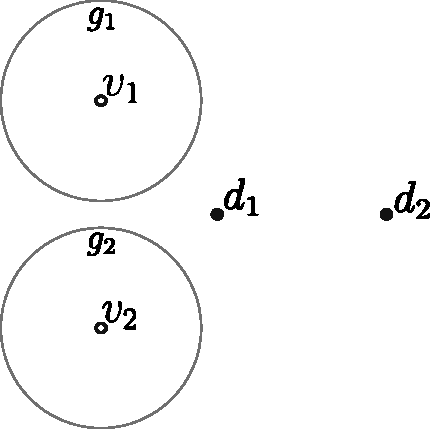
\includegraphics[width=1.0\columnwidth]{assets/fcm_problem.pdf} 
      \caption{Problema dos ruídos} 
      \label{fig:fcm_problem} 
    \end{figure}
  \end{columns}
\end{frame}

\begin{frame}{Agrupamento (PCM) \cite{Krishnapuram1993}}
  \begin{columns}
    \column{0.5\textwidth}
    \begin{itemize}
      \item Graus de tipicidade. 
      \item Problema dos grupos coincidentes. 
      \item \alert{Remoção da restrição probabilística}.
    \end{itemize} 
    \begin{table}[!htp]
      \centering
      \begin{tabular}{ |l|c|c|c|}
        \hline
        & {\bf$grupo_1$} & {\bf $grupo_2$} & {\bf \alert{total}} \\
        \hline
        $doc_1$ & 0,7 & 0,7 & 1,4 \\
        \hline
        $doc_2$ & 0,2 & 0,2 & 0,4 \\
        \hline
      \end{tabular}
      \caption{Tipicidades PCM}
    \end{table}

    \column{0.5\textwidth}
    \begin{figure}[!htp] \centering
      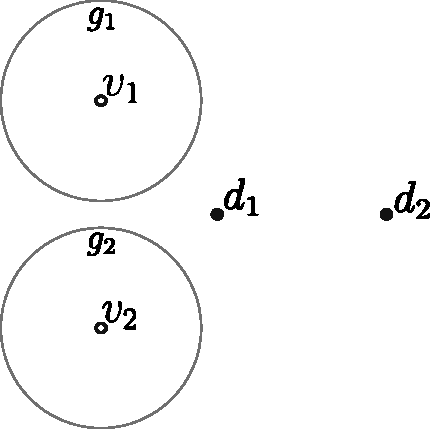
\includegraphics[width=1.0\columnwidth]{assets/fcm_problem.pdf} 
      \caption{Problema dos ruídos} 
      \label{fig:fcm_problem} 
    \end{figure}
  \end{columns}
\end{frame}

\begin{frame}{Agrupamento (PFCM) \cite{Pal2005}}
  \begin{columns}
    \column{0.5\textwidth}
    \begin{itemize}
      \item Pertinências e tipicidades. 
      \item Robustez. 
      \item Parâmetros de ponderação $a$ e $b$.
    \end{itemize} 

    \begin{figure}[!htp] 
      \centering 
      \includegraphics[width=1.0\columnwidth]{assets/samples_pfcm.png}
      \caption{Agrupamento de pontos.} 
      \label{fig:samples_pfcm} 
    \end{figure}

    \column{0.5\textwidth}
    \begin{table}[!htp]
      \centering
      \begin{tabular}{ |l|c|c|c|}
        \hline
        & {\bf$grupo_1$} & {\bf $grupo_2$} & {\bf total} \\
        \hline
        $doc_1$ & 0,50 & 0,5 & 1,0 \\
        \hline
        $doc_2$ & 0,5 & 0,5 & 1,0 \\
        \hline
      \end{tabular}
      \caption{Pertinências PFCM}
    \end{table}
    \begin{table}[!htp]
      \centering
      \begin{tabular}{ |l|c|c|c|}
        \hline
        & {\bf$grupo_1$} & {\bf $grupo_2$} & {\bf total} \\
        \hline
        $doc_1$ & 0,7 & 0,7 & 1,4 \\
        \hline
        $doc_2$ & 0,2 & 0,2 & 0,4 \\
        \hline
      \end{tabular}
      \caption{Tipicidades PFCM}
    \end{table}
  \end{columns}
\end{frame}

\subsection{Extração de descritores}
\begin{frame}{What is haplotyping and why is it important?}
  You hopefully know this after the previous three talks\dots
\end{frame}

\section{Trabalhos relacionados}

\begin{frame}{What is haplotyping and why is it important?}
  You hopefully know this after the previous three talks\dots
\end{frame}

\section{Abordagem proposta}

\subsection{Refinamento com PFCM}
\begin{frame}{What is haplotyping and why is it important?}
  You hopefully know this after the previous three talks\dots
\end{frame}
\subsection{Método PDCL}
\begin{frame}{What is haplotyping and why is it important?}
  You hopefully know this after the previous three talks\dots
\end{frame}
\subsection{Método Mixed-PFDCL}
\begin{frame}{What is haplotyping and why is it important?}
  You hopefully know this after the previous three talks\dots
\end{frame}

\section{Conclusão}

\begin{frame}{What is haplotyping and why is it important?}
  You hopefully know this after the previous three talks\dots
\end{frame}

\section{Trabalhos futuros}

\begin{frame}{What is haplotyping and why is it important?}
  You hopefully know this after the previous three talks\dots
\end{frame}

%\begin{frame}
%Quais seriam as possíveis histórias do tráfico atlântico?
%  \frametitle{Introdu\c{c}\~{a}o}
%    \begin{enumerate}
%        \justifying
%      \item Uma história \textbf{apenas} com os documentos europeus.
%      \item Uma história \textbf{sem} eles -- entraves metodológicos e
%        epistemológicos.\footnote{\justifying VANSINA, Jan. Oral tradition and its methodology
%        \textit{UNESCO General History of Africa}. v.1. Methodology and African History. Berkeley:
%      University of California Press, 1981, p.54-61. LAW, Robin. \textit{The kingdom of Allada}.
%    Leiden: Research School CNWS, School of Asian, African, and Amerindian Studies, 1997. HIRSCH,
%  Eric; STEWART, Charles. Introduction: Ethnographies of Historicity. In: \textit{History and
%Anthropology}, v.16,n.3, p.261-274, 2005.\\}
%      \item Uma história a partir dos documentos mencionados e daqueles que foram produzidos por
%        africanos e africanas, incluindo a ``voz'' que se encontra encapsulada nos documentos
%        europeus -- o que pretendemos demonstrar.
%    \end{enumerate}
%  \end{frame}

  \begin{frame}{Introdução}
%  \frametitle{Introdu\c{c}\~{a}o}
%  \begin{itemize}
%      \justifying
%      \item Provocações da antropologia pós-moderna: contra o papel pretensamente colonial da disciplina e da predominância da autoridade centrada na ``voz'' do pesquisador : pertinências e exageros. \footnote{\justifying CLIFFORD, James; MARCUS, George E. \textit{Writing Culture}: The Poetics and Politics of Ethnography. 3.ed.  2010.}
%      \item ``Caminho do meio'' entre esse discurso e nosso propósito aqui hoje: Bakhtin. 
%      \item Contribuição dos conceitos bakhtinianos de polifonia e dialogismo: irredutibilidade do discurso a um único ``emissor''.\footnote{\justifying BAKHTIN, Mikhail. \textit{Problems of Dostoevsky’s Poetics}. Tradução Caryl Emerson. Minneápolis: University of Minnesota, 1984.}
%      \item Uma perícia acurada permite buscar reversões do encapsulamento, conceito muito caro o certos ramos da ciência da computação.
%  \end{itemize}  
\end{frame}

%\begin{frame}
%      \justifying Indícios de validade histórica dos diálogos pretensamente transcritos pelos europeus:
%  \frametitle{Introdu\c{c}\~{a}o}
%  \begin{enumerate}
%    	\justifying
%      \item Palavras transliteradas de línguas africanas consideradas procedentes pelos seus falantes e estudiosos.
%      \item Descrições etnográficas posteriores com informações muito semelhantes.
%  \end{enumerate} 
%  Versavam sobre muitos assuntos, porém, em geral, os interlocutores da África eram preferencialmente europeizados. 
%\end{frame}
%
%\section{Os devoradores da vida e da riqueza}
%\begin{frame}
%  \frametitle{Os devoradores da vida e da riqueza}
%  \begin{itemize}
%  	\justifying
%	\item Entre as muitas versões desses diálogos, um capitão inglês teria colhido relatos africanos de que eles acreditavam que seriam devorados por feiticeiros brancos após a viagem pelo mar.\footnote{PHILLIPS, Thomas. A  journal of a voyage made in ... 1693, 1694 ... to Africa. In: VÁRIOS. \textit{ A Collection of voyages and travels...}. vol.6. Londres: Churchill and Churchill, 1735, p.173-239. p.215}
%	\item Validação etnográfica contemporânea: o ato de devorar é uma metanarrativa de um poder violento.\footnote{\justifying SHAW, Rosalind. The Production of Witchcraft/Witchcraft as Production: Memory, Modernity, and the Slave Trade in Sierra Leone. In: \textit{The American Ethnologist}, Blackwell Publishing on behalf of the American Anthropological Association Stable, vol. 24, n.4, p.856-876, 1997. WEST, Henry. \textit{Kupilikula}: governance and the Invisible Realm in Mozambique. 2ed. Chicago: University of Chicago Press, 2005. GESCHIERE, Peter.  Witchcraft and Modernity: Perspectives from Africa and Beyond. In: PARÉS, Luis Nicolau; SANSI, Roger (ed.). \textit{Sorcery in the Black Atlantic}. Chicago: University Chicago Press, p.233-258, 2011.}
%  \end{itemize}
%\end{frame}
%
%\section{A percepção sobre o impacto destrutivo}
%\begin{frame}
%  \frametitle{A percepção sobre o impacto destrutivo}
%      \justifying
%      \begin{itemize}
%      \justifying
%      \item A memória oral preservou narrativas sobre o medo de raptos e vendas no litoral e sobre europeus ``tomavam conta'' de crianças em certos lugares.\footnote{\justifying BAILEY, Anne C. \textit{African voices of the Atlantic slave trade}: beyond the silence and the shame. Beacon Press: Boston, 2005. p.164-170 }
%      \item O rei Agajá daomeano teria mencionado interesse em comercializar outros bens em lugar de vender pessoas, e um grande interesse em aprender a tecnologia dos brancos. Uma evidência de factibilidade dessa carta seria um trecho em que o rei expressa repulsa pela monogamia dos europeus. Isso é muito recorrente nos diálogos entre líderes africanos e os europeus.\footnote{\justifying ROBIN, Law. An Alternative Text of King Agaja of Dahomey's Letter to King George I of England, 1726. In:   \textit{History in Africa}, v.29, p.257-271. }
%      \end{itemize}
%\end{frame}
%
%\begin{frame}
%  \frametitle{A percepção sobre o impacto destrutivo}
%      \justifying
%      \begin{quotation}
%The discerning Natives account it their greatest Unhappiness, that they were ever visited by the Europeans. They say, that we Christians introduc’d the Traffick of Slaves, and that before our Coming they liv’d in Peace; but,  say they, it is observable, that where-ever Christianity comes, there come with it a Sword, a Gun, Powder and Ball. \footnote{\justifying SMITH, William. New voyage to Guinea […]. Londres: J. Nourse, 1744. p.266.\\}
%      \end{quotation}
%\end{frame}
%
%\section{Conclusões}
%\begin{frame}
%  \frametitle{Conclusões}
%    \begin{itemize}
%        \justifying
%      \item O estudo crítico permite buscar a ``voz'' africana encapsulada nos registros europeus.
%      \item As interpretações metafóricas dos traficantes europeus compreendidos como feiticeiros canibais encontra ressonância em outras evidências etnográficas.
%      \item As críticas aos significados políticos e aos impactos econômicos encontram sustentação metodológica nas evidências culturais circundantes, seja nos estudos linguísticos ou na antropologia.
%      \item Novas pesquisas a partir fontes inéditas e das já conhecidas, sob um novo olhar agora, viabilizarão uma história do tráfico atlântico tendo como alvo o ponto de vista das africanas e dos africanos.
%    \end{itemize}
%  \end{frame}

\bibliographystyle{abntex2-alf}
\bibliography{biblio}

\end{document}
